%  DOCUMENT CLASS
% \documentclass[a4paper,12pt,twoside,chapterprefix=false]{scrreprt}
\documentclass[a4paper,12pt,oneside,chapterprefix=false]{scrreprt}
%PACKAGES
\usepackage[latin1]{inputenc}  % Quelltext ist ISO-8859-1 codiert
\usepackage[ngerman]{babel}
\usepackage[reqno,fleqn]{amsmath}
\setlength\mathindent{10mm}
\usepackage{amssymb}
\usepackage{amsthm}
\usepackage{amsfonts}
% \usepackage{extarrows}
\usepackage{fancyhdr}
\usepackage{units}
%\usepackage{fourier,eurosym} funktioniert nicht auf Physnet-Rechnern
\usepackage{fourier, eurosym}
\usepackage{syntax}
\usepackage{amstext}    % defines the \text command
\usepackage{array}
\usepackage{graphicx}
\usepackage{subfigure}
\usepackage{wrapfig}


% FORMATIERUNG
\usepackage[paper=a4paper,left=30mm,right=25mm,top=30mm,bottom=35mm]{geometry}
\setlength{\parindent}{0cm}
\setlength{\parskip}{1.5mm plus1mm minus1.5mm}
\addtokomafont{sectioning}{\rmfamily}

%-zusaetzliche Kommandos und Abkuerzungen aus externer Datei

\newcommand*{\NN}{\mathbb N}  %Natuerliche Zahlen
\newcommand*{\ZZ}{\mathbb Z}  %Ganze Zahlen
\newcommand*{\RR}{\mathbb R}  %Reelle Zahlen
\newcommand*{\CC}{\mathbb C}  %Komplexe Zahlen
\newcommand*{\eps}{\varepsilon}  %Komplexe Zahlen


\begin{document}
% Seitennummerierung f�r Titel, Widmung, Danksagung, Zusammenfassung
% und Inhaltsverzeichnis werden in roemischen Zahlen gesetzt
% \renewcommand{\thepage}{\roman{page}} % Roman page numbers

% Titelblatt
\begin{titlepage}

\title{
  \Large{\textbf{
    Universit�t Hamburg\\
    Physikalisches Praktikum f�r Fortgeschrittene\\
    Sommersemester 2014
  }}\\
  \vspace{8cm}
  \huge{\textbf{
    Versuch:\\Laserspektroskopie an Rubidium
  }}
}

\author{
  \large
  \vspace{4cm}
  \begin{tabular}{ll}
  Praktikanten:
  &Alexander Okupnik\\
  &Vincent Koppen\\
  Betreuer:\quad&Dr. Matthias �lschl�ger\\
  \end{tabular}
}

\date{\large{
    durchgef�hrt vom 8.9. bis zum 10.9.2014
  }}

\end{titlepage}

\maketitle

% Inhalts-, Abbildungs*-, Tabellen*-Verzeichnis
\tableofcontents
% \newpage

% \renewcommand{\thepage}{\arabic{page}} % Arabic page numbers
% \setcounter{page}{1}

% Kapitel
\chapter{Theoretische Grundlagen}


\section{Energie�berg�nge in Rubidium} \label{sec:linien}

In diesem Versuch wird Rubidium (Atomnummer 37) spektroskopisch untersucht.
Rubidium hat die stabilen Isotope $^{85}\text{Rb}$ mit der H�ufigkeit 72\% und
$^{87}\text{Rb}$ mit der H�ufigkeit 28\%. Als Alkalimetall verh�lt es sich �hnlich
wie Wasserstoff, die ersten 36 Elektronen sind in abgeschlossenen H�llen und es
gibt nur ein Valenzelektron, das zum Gesamtspin $\frac{1}{2}$ beitr�gt. Die
ersten angeregten Zust�nde dieses Elektrons --
wenn also $l=1$ ($l$: Bahndrehimpulsquantenzahl) -- sind zun�chst zwei durch
die Spin-Bahn-Kopplung getrennte Zust�nde mit $J=\frac{1}{2}$ und $J=\frac{3}{2}$:
die sogenannten D1- und D2-Linien ($J$: Gesamtdrehimpulsquantenzahl).
Wir untersuchen im Folgenden nur die D2-Linie,
die einer Lichtwellenl�nge von 780 nm entspricht.

\begin{figure}[ht]
  \center
  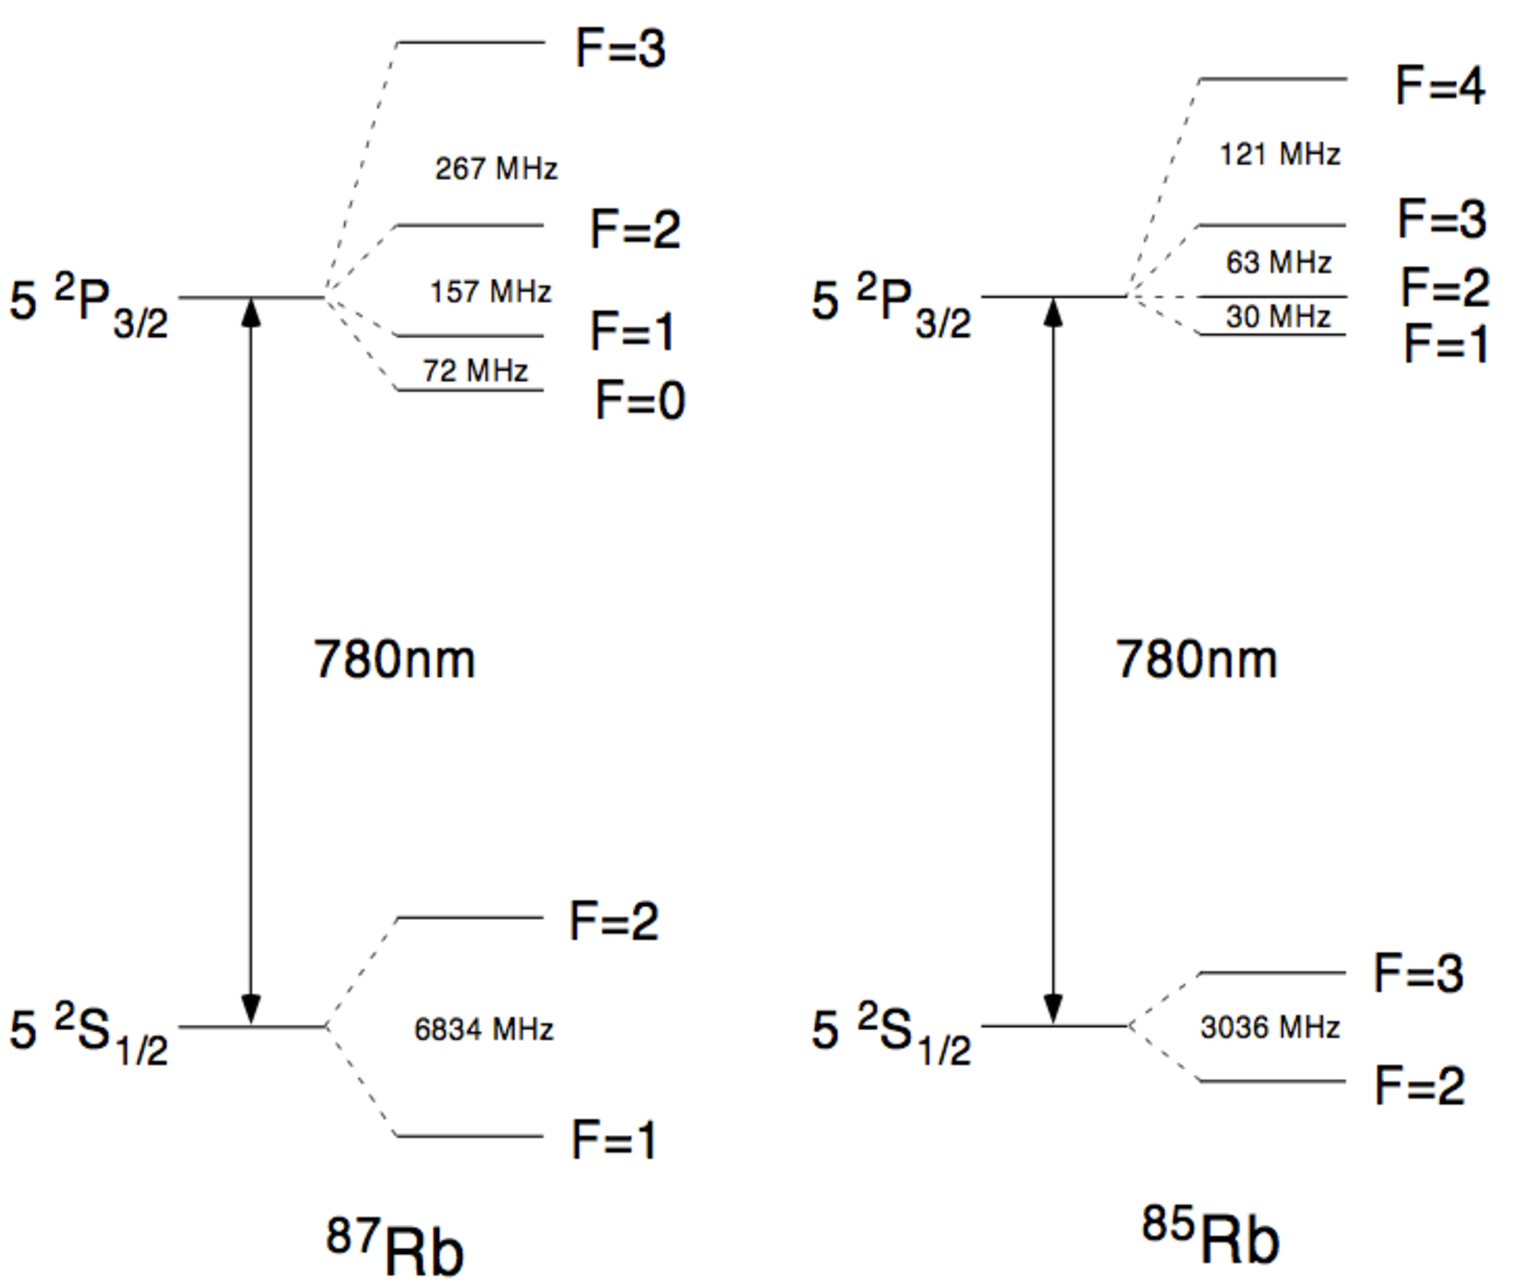
\includegraphics[width=0.85\textwidth]{./Rb-D2-Hyperfein.pdf}
  \caption{Hyperfeinstruktur der D2-Linie der Isotope $^{85}\text{Rb}$ und
  			$^{87}\text{Rb}$ ([1])}
	\label{fig:rbd2hyperfein}
\end{figure}

Die Interaktion des H�llendrehimpuls des Rubidium-Atoms mit seinem Kernspin f�hrt
zur Aufspaltung der D2-Linie, und zwar unterschiedlich f�r die beiden Isotope:
$^{85}\text{Rb}$ hat Kernspin $\frac{5}{2}$ und $^{87}\text{Rb}$ $\frac{3}{2}$.
Es gibt nun alle Energie�berg�nge in Abbildung \ref{fig:rbd2hyperfein} zu beobachten,
die $\Delta$F$=0,\pm1$ erf�llen, wobei $F$ die Quantenzahl der Summe
von Kernspin und H�llendrehimpuls ist. Wir werden im ersten Teil des Versuchs
nur vier verschiedene �berg�nge aufl�sen k�nnen -- f�r die zwei Isotope jeweils
die beiden �berg�nge von den zwei Grundniveaus (vgl. Abbildung \ref{fig:rbd2hyperfein}).
Die vier verschiedenen angeregten Niveaus je Isotop liegen energetisch im Vergleich
zu allen anderen wesentlich n�her aneinander und werden erst im zweiten Versuchsteil
experimentell zu beobachten sein.

\section{Linienverbreiterung}

\subsection{Nat�rliche Linienbreite und S�ttigungsverbreiterung}
Die sogenannte nat�rliche Linienbreite entsteht wegen der Energie-Zeit-Unsch�rferelation
aus der Zeitbegrenztheit der Lebensdauer der angeregten Atomzust�nde. Sie hat
die Form eines Lorentzprofils.

Wir betrachten in diesem Versuch mit dem Rubidium-Gas ein Vielteilchensystem
aus Alkali-Atomen (mit einer charakteristischen S�ttigungsintensit�t
$I_{\text{sat}}$), die f�r feste Frequenzen einwirkenden
Lichts als Zwei-Niveau-Systeme betrachtet werden k�nnen. Wenn dieses
mit einem monochromatischen nahresonanten Laserfeld der Intensit�t $I$
wechselwirkt, dann ist die Anregungswahrscheinlichkeit der Atome
\begin{equation} \label{eq:lorentz}
	\rho = \frac{1}{2}\frac{s}{\delta^2+(\frac{\Gamma}{2})^2} \text{ .}
\end{equation}

Hier ist $\delta$ der Frequenzabstand des Laserlichts von der \emph{eigentlichen}
�bergangsfrequenz im Sinne der Linien
aus Abschnitt \ref{sec:linien}, $s := \frac{I}{I_{\text{sat}}}$ der Intensit�tsparameter
und
$\Gamma$ (die volle Halbwertsbreite von \eqref{eq:lorentz}) eine in Abh�ngigkeit
der Intensit�t durch den Effekt der S�ttigungsverbreiterung vergr��erte Version der
nat�rlichen Linienbreite $\gamma$.

Die S�ttigungsverbreiterung kommt dadurch zustande,
dass bei erh�hter einfallender Intensit�t die Lebensdauer des angeregten Zustands,
dessen Zerfall sich aus spontaner und stimulierter Emission zusammensetzt, wegen
erh�hter Rate stimulierter Emission verringert wird. Hieraus ergibt sich wegen der
Energie-Zeit-Unsch�rferelation eine Verbreiterung der
Anregungswahrscheinlichkeitsverteilung.
		\begin{comment}
		der Grundzustand st�rker entv�lkert wird
		und damit die Anregungswahrscheinlichkeit sinkt, und zwar umso mehr, je gr��er die
		Absorptionswahrscheinlichkeit im Vornhinein war. Insgesamt verbreitert sich also
		die Anregungswahrscheinlichkeitsverteilung.
		\end{comment}
		
In unserem Versuchsaufbau wird eine S�ttigung durch zwei Strahlen aus verschiedenen
Richtungen und unter Anderem dadurch stattfindende Umpumpprozesse daf�r sorgen,
dass die Leistungsverbreiterung der nat�rlichen Linienbreite durch den Faktor 
$1+\sqrt{1+s}$ beschrieben wird, d.h.
\begin{equation} \label{eq:mitformel}
	\Gamma = \gamma(1+\sqrt{1+s}).
\end{equation}

F�r Herleitungsans�tze sei auf [2] verwiesen.


\subsection{Dopplerverbreiterung}

Dar�ber hinaus gibt es eine weitere Art der Verbreiterung der gemessenen
Absorptionslinien, wenn ein Gas aus Atomen der Masse $m$ mit Temperatur $T$
spektroskopiert wird.
In ihrem Ausma� dominiert diese bei Raumtemperatur die oben diskutierten Breiten,
was wir im ersten Versuchsteil beobachten werden und mit der Methode,
die wir im zweiten Versuchteil kennen lernen, umgehen k�nnen.

Die Projektionen der Geschwindigkeiten der Atome auf die Richtung des Laserlichts
folgen nach Maxwell-Boltzmann einer Normalverteilung um 0 mit der vollen Halbwertsbreite
$2 \sqrt{\frac{2\ln2k_BT}{m}}$. Wegen des
Doppler-Effekts ist daher die Verteilung der Frequenzen von Photonen, die auf
einzelne Atome wirken, jeweils aus Sicht des getroffenen Atoms genommen, eine
Normalverteilung um die Laserfrequenz im Laborsystem mit der vollen Halbwertsbreite
\begin{equation}
	\Delta \nu = 2 \frac{1}{\lambda} \sqrt{\frac{k_B T}{m}2\ln{2}} \ .
\end{equation} \label{eq:gausstemp}
Hierbei ist $\lambda$ die der jeweiligen Frequenz entsprechende
Wellenl�nge der Laserlichts.
Bei der Spektroskopie des Gases entsteht diese Verteilung jeweils um die
Anregungsfrequenzen als Form der gemessenen Spektrallinien.

Da sich hieraus f�r Rubidium bei Raumtemperatur Breiten ca. �ber 500 MHz
ergeben und die nat�rliche Linienbreite bei nur 6 MHz liegt, werden wir
im Versuch im Falle einer Dopplerverbreiterung von einer reinen 
Normalverteilung ausgehen, w�hrend man pr�ziser eine Faltung des
Lorentzprofils der nat�rlichen Linienbreite mit der Normalverteilung
durch den Dopplereffekt betrachten m�sste.


\section{Dopplerfreie S�ttigungsspektroskopie}

Wegen der oben erkl�rten Dopplerverbreiterung, die bei Raumtemperatur die
Abst�nde der
verschiedenen �berg�nge zwischen einem Grundniveau eines der beiden Isotope
und den verschiedenen angeregten Niveaus �berragt, werden wir mit einem 
konventionellen Experiment nicht alle
Linien der Hyperfeinstruktur aus Abbildung \ref{fig:rbd2hyperfein} aufl�sen
k�nnen.

Es gibt eine Methode, bei der man Rubidium-Gas bei Raumtemperatur
absorptionsspektroskopiert, mit der man das kann, die im Folgenden beschrieben wird.

Dem Teststrahl, der das Gas von einer Seite durchdringt
(und von dem im ersten Versuchsteil schlicht die Transmission
aufgenommen wird) wird ein weiterer sogenannter Pumpstrahl mit gleicher
Frequenz hinzugef�gt,
der das Gas von der anderen Seite trifft und mit dem Teststrahl �berlappt.
Der Pumpstrahl hat eine so hohe Intensit�t, dass er die Grundzust�nde von
Atomen, die er mit seiner Frequenz und deren Geschwindigkeit anregen kann,
im Wesentlichen entv�lkert. Wenn nun die Laserfrequenz
keiner Anregungsfrequenz (im Rahmen der pumpstrahls�ttigungsverbreiterten
nat�rlichen Linienbreite)
gleich ist, dann regen Pump- und Teststrahl (fast immer, beachte
Crossover-Resonanzen) unterschiedliche
Geschwindigkeitsklassen von Atomen an (wenn �berhaupt), und daher bleibt dort
das dopplerverbreiterte Spektrum aus dem ersten Versuchsteil unver�ndert.
Wenn die Laserfrequenz eine Anregungsfrequenz trifft, dann werden die 
Grundzust�nde der projiziert auf die Laserstrahlen ruhenden Atome durch den
Pumpstrahl entv�lkert und der Teststrahl wird transmittiert, anders als im reinen
dopplerverbreiterten Spektrum und wird dem Transmissionspektrum daher hinzugef�gt.
Die durch die
Zimmertemperatur verursachte Dopplerverbreiterung wird hier also durch die Bedingung,
dass die entsprechenden Atome Geschwindkeit 0 in Richtung des Laserlichts haben,
aufgehoben.
Zus�tzlich zu den so aufgel�sten Linien mit nur leistungsverbreiterter nat�rlicher
Linienbreite beobachtet man bei Systemen mit mehr als einem Anregungsniveau
nun noch die sogenannten \emph{Crossover}-Resonanzen mit
gleicher Breite, die in der Mitte zwischen zwei echten Resonanzen auftreten.
Verursacht sind sie dadurch, dass es bei Laserfrequenzen, die genau zwischen
(und im Gegensatz zur Dopplerverbreiterung nah bei) zwei
verschiedenen Anregungsfrequenzen liegen, Geschwindigkeitsklassen von Atomen
gibt, die der Teststrahl aufgrund Blau- bzw. Rotverschiebung anregen w�rde, die
der Pumpstrahl aber wegen entsprechender Rot- bzw. Blauverschiebung auch anregen kann,
dies auch tut und den verantwortlichen Grundzustand entv�lkert, sodass der Teststrahl
wie bei den echten Resonanzfrequenzen auch transmittiert wird.


\section{Messmethoden}

\subsection{Fabry-P�rot-Interferometer}

Ein Fabry-P�rot-Interferometer oder -Resonator dient unter Anderem zur Kalibrierung
von Frequenzdifferenzen. Es besteht prinzipiell aus zwei parallelen Endplatten,
die au�en schwach reflektieren und deren Innenseiten stark reflektieren.
Monochromatisches Licht,
das in die eine Seite einf�llt und aus der anderen austritt, wird im Interferometer
unterschiedlich oft hin- und herreflektiert und das insgesamt austretende Licht
ist eine �berlagerung davon. Es ist also intensiv bei Frequenzen, die zur
Bildung von stehenden Wellen im Interferometer f�hren, und sonst verschwindend,
da das unterschiedlich lang im Interferometer gewesenene Licht dann destruktiv
interferiert. Die Abst�nde zwischen den Frequenzen,
bei denen sich stehende Wellen ausbilden, sind konstant und h�ngen von der L�nge
und dem Brechungsindex des Resonators ab [2]. Ersteres werden wir im Versuch
ausnutzen. Die Resonanzen, die man hinter dem Resonator bei bestimmten Frequenzen
beobachtet, haben wegen der endlichen Lebensdauer der Photonen innerhalb
des Resonators eine gewisse endliche Breite.

\subsection{Intensit�t und Leistung des Laserstrahls}

Wir nehmen an, dass die Intensit�t des im Versuch verwendeten Laserstrahls entlang
transversaler Richtungen gau�verteilt ist mit den halben $\frac{1}{e^{2}}$--Breiten
$w_x$ und $w_y$ in horizontaler bzw. vertikaler Richtung:
\begin{equation}	\label{eq:intensitaet}
	I(x,y) =
	I_0 \exp{\left(-\frac{2x^2}{w_x^2}\right)} \exp{\left(-\frac{2y^2}{w_y^2}\right)}
\end{equation}

F�r die Leistung $P$ des Laserstrahls gilt dann
\begin{equation}
	P = \int_{-\infty}^{\infty} \int_{-\infty}^{\infty}
		I_0
		\exp{\left(-\frac{2x'^2}{w_x^2}\right)} \exp{\left(-\frac{2y'^2}{w_y^2}\right)}
		dx' dy'
	  = \frac{\pi}{2} w_x w_y I_0	\nonumber
\end{equation}
und somit, wenn man dem Strahl der Einfachheit halber \emph{einen} Wert $I$ f�r die
Intensit�t zuordnet
und daf�r das Intensit�tsmaximum $I_0$ in der Strahlmitte w�hlt,
\begin{equation}	\label{eq:intensitaetleistung}
	I = \frac{2P}{\pi w_x w_y} \text{ .}
\end{equation}
Dies f�hrt nat�rlich zu einer �bersch�tzung der Intensit�t, wenn man die Leistung des
Strahls misst, wie wir es in diesem Versuch tun.

Wenn der Strahl mit Intensit�t nach \eqref{eq:intensitaet} von einer Seite aus vertikaler
Richtung durch eine Klinge mit horizontaler Kante -- mit vertikaler Position $y$ relativ
zur Strahlmitte (das Vorzeichen sei in die Richtung, in die sie hineingeschoben wird) --
abgedeckt wird, dann ist die �brigbleibende Leistung
\begin{equation} \label{eq:yerrfct}
	\begin{split}
	P_y &= \int_y^{\infty} \int_{-\infty}^{\infty}
		I_0
		\exp{\left(-\frac{2x'^2}{w_x^2}\right)} \exp{\left(-\frac{2y'^2}{w_y^2}\right)}
		dx' dy' \\
	  &= I_0
	  \left(\int_{-\infty}^{\infty} \exp{\left(-\frac{2x'^2}{w_x^2}\right)} dx' \right)
	  	\frac{\sqrt{\pi}w_y}{2\sqrt{2}}
		\left( 1-\text{erf}
		 \footnotemark\left(\frac{\sqrt{2}y}{w_y}\right) \right) \\
	  &\propto 1-\text{erf}\left(\frac{\sqrt{2}y}{w_y}\right)
	\end{split}
\end{equation}
\footnotetext{erf$(x) := \frac{2}{\sqrt{\pi}} \int_0^x \exp{(-t^2)}\,dt
	\ \text{ f�r }x\in\mathbb{R}$}
und analog gilt f�r die Leistung bei einer vertikalen Klinge aus horizontaler Richtung

\begin{equation} \label{eq:xerrfct}
	P_x \propto 1-\text{erf}\left(\frac{\sqrt{2}x}{w_x}\right) \text{.}
\end{equation}
\chapter{Versuchaufbau/Durchf�hrung}
\section{Dopplerspektroskopie}

\begin{figure}[ht]
 \center
  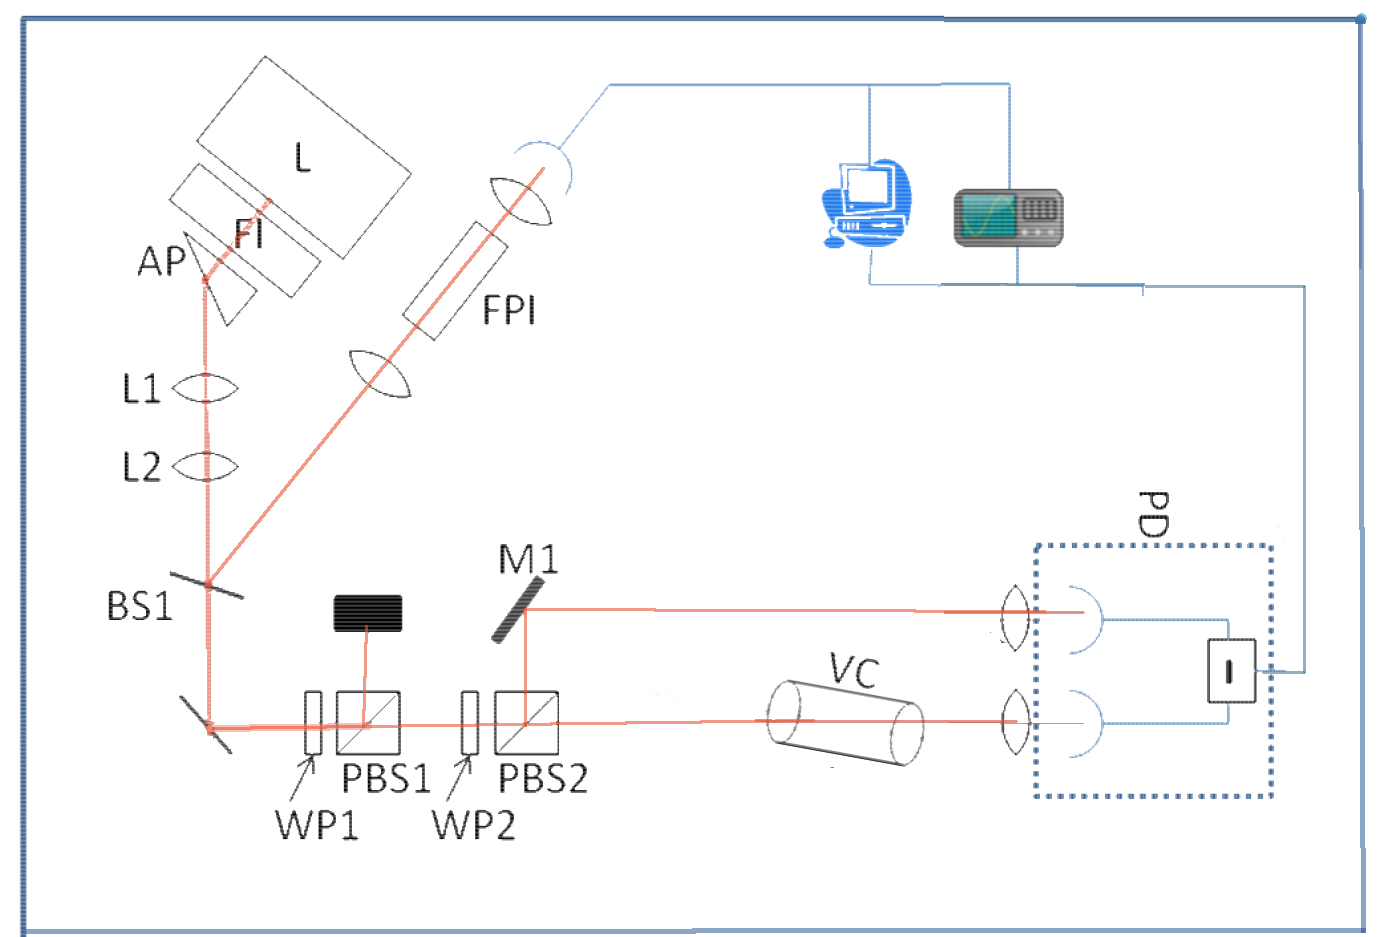
\includegraphics[width=0.85\textwidth]{./aufbau.png}
  \caption{Schematischer Aufbau Dopplerspektroskopie}
\end{figure}
Der Laserstrahl trifft durch eine Faraday-Diode (FI) auf ein Prisma (AP), welches die elliptischen Strahlform korrigiert. 

Die Faraday-Diode soll R�ckreflexionen auf die Laserquelle blockieren um daraus resultierende St�rquellen zu vermeiden. 
An dem Strahlteiler BS1 wird ein Teil des Strahles reflektiert , durch einen Fabry-P�rot-Interferometer in eine Photodiode geworfen. 
Da das FPI nur in gleichen diskreten Frequenzabschnitten einfallendes Licht wieder aussendet kann man damit den Frequenzbereich, 
den der Laser abf�hrt skalieren.

Der Hauptteil des Strahles mit dem wir experimentieren werden wird von einem Spiegel
reflektiert und durch ein \( \frac{\lambda}{2} \)-Pl�ttchen (WP1) auf ein Polarisationsstrahlteiler (PBS1) geschickt.

Der PBS reflektiert s-polarisiertes Licht und l�sst p-polarisiertes Licht transmittieren. 

Drehen wir am \( \frac{\lambda}{2} \)-Pl�ttchen das Intensit�tsverh�ltnis der beiden Strahlen und k�nnen damit die Intensit�t des p-polarisierten Strahles deutlich absenken.

Dieser Strahl trifft nochmal auf ein WP/PBS Paar und wird in 2 Strahlen gleicher Intensit�t aufgeteilt. 
Der Teststrahl trifft auf die Rubidiuumzelle und wird teilweise absorbiert, teilweise transmittiert er. 
Der Referenzstrahl trifft dann zusammen mit dem Teststrahl auf eine differentielle Photodiode. 
Die in Ihr absorbierten Strahlen werden in Spannungen umgewandelt und voneinander abgezogen, sodass man 
als resultierende Spannung am Oszilloskop das absorbierte Spektrum sehen kann.


In der Versuchsdurchf�hrung haben wir uns am Oszilloskop zun�chst das Signal am FPI angeguckt ob wir saubere Peaks zu sehen bekommen,
teilweise war der Untergrund etwas verrauscht und man hatte neben den Hauptpeaks kleinere Nebenpeaks. Das ist ein Hinweis darauf, 
dass der Laser nicht nur monochromatisches Licht aussendet und dies kann behoben werden indem man dem Strom des Lasers variiert. 
Der Wellenl�ngenbereich in dem der Laser Strahlung emittiert wurde solange variiert bis man die erwarteten 4 dopplerverbreiteten 
Emissionspeaks zu sehen bekam. 

Beide Signale wurden aufgenommen und mit Origin verwertet, N�heres dazu wird in der Auswertung erl�utert. 

\section{Dopplerfreie Spektroskopie}

\begin{figure}[ht]
 \center
  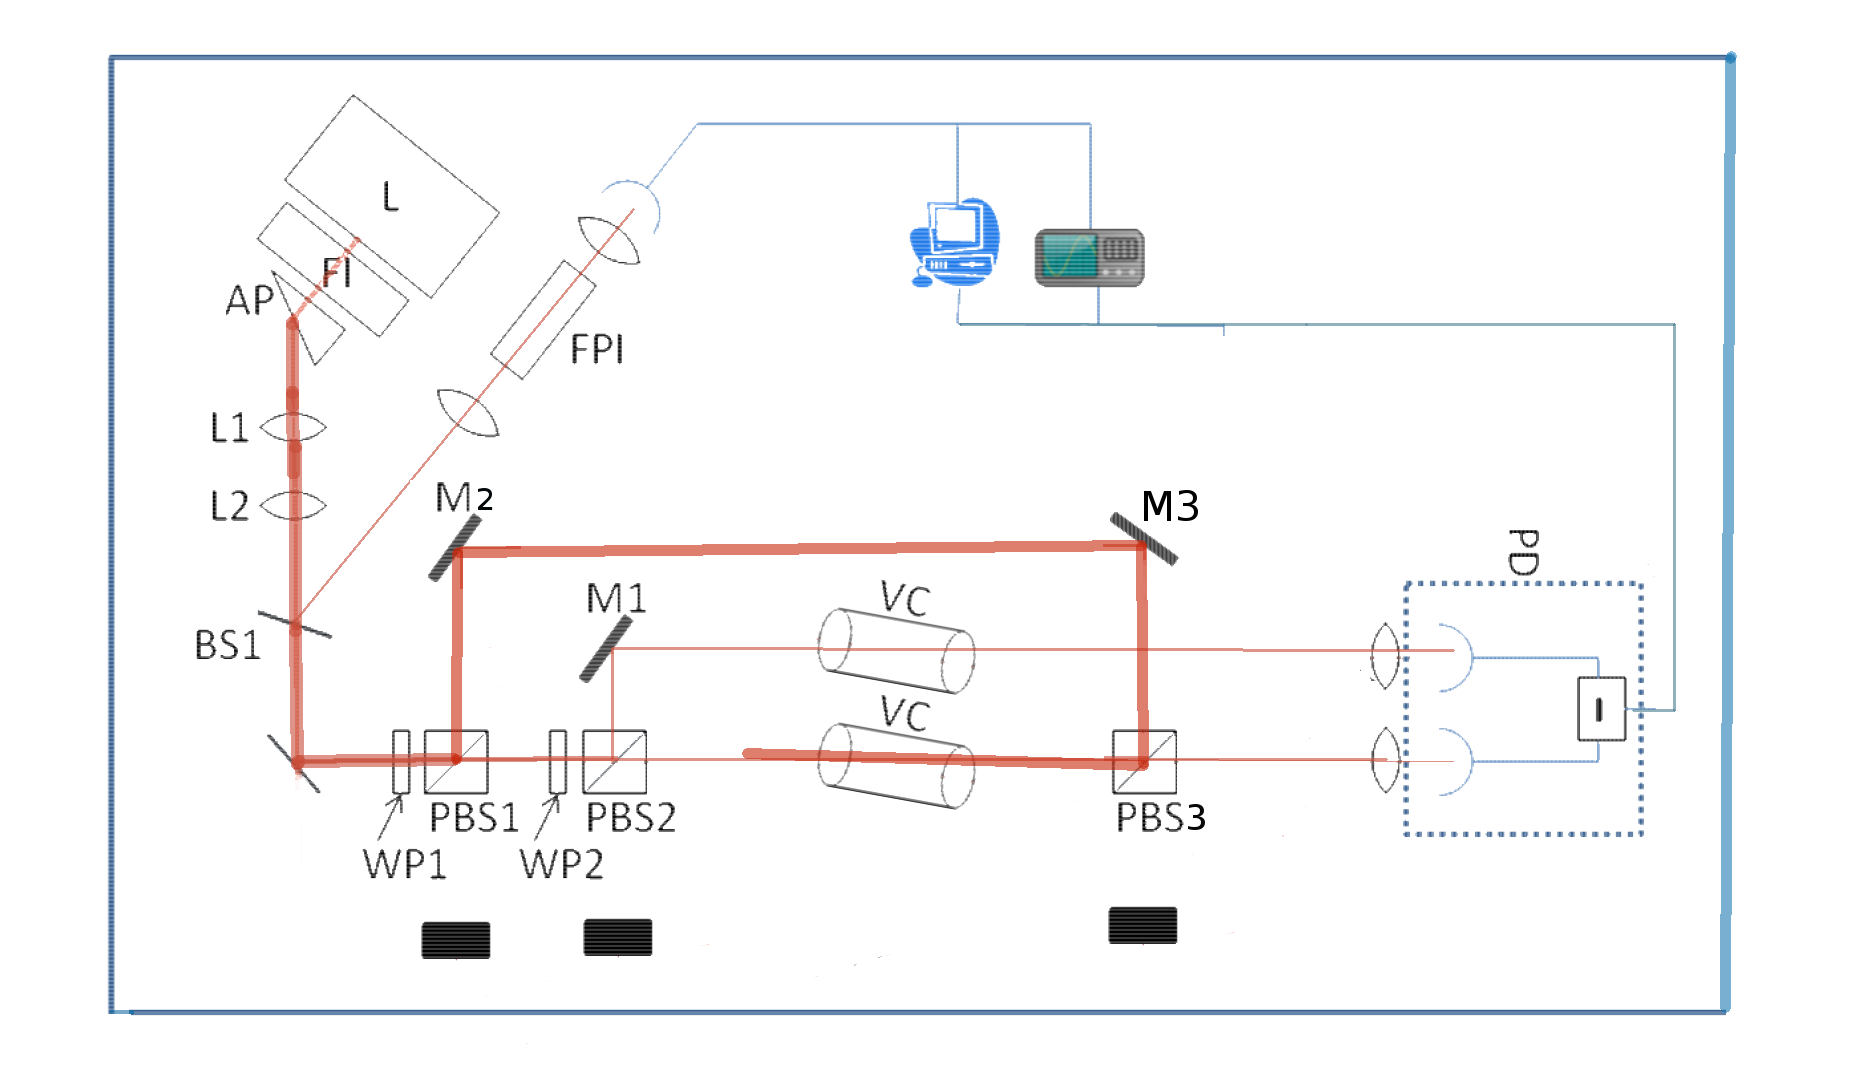
\includegraphics[width=0.85\textwidth]{./Dopplerfrei.png}
  \caption{Schematischer Aufbau der dopplerfreien Spektroskopie}
\end{figure}

Im zweiten Versuchsteil haben wir den selben Aufbau verwendet und etwas modifiziert. 

Anstatt den p-polarisierten Strahl am PBS1 abzublocken, nutzt man die um Gr��enordnungen
h�here Intensit�t als Pumpstrahl. Er soll m�glichst auf der gleichen Geraden wie der Teststrahl durch die Rubidiumzelle 
laufen um die zu messenden Hyperfeinstrukturlinien zu s�ttigen. 

Daf�r wird der Strahl mit zwei Spiegeln auf PBS3 geworfen der mittig in die Bahn des Teststrahles zwischen Zelle und Photodiode
positioniert wird. Den Pumpstrahl l�sst er transmittieren oder reflektiert ihn auf die Teststrahlgerade, je nach dem wie er polarisiert ist.

Den Teststrahl l�sst er im Idealfall unber�hrt transmittieren, da er bereichts durch PBS2 p-polarisiert ist.

Mit einem weiteren \( \frac{\lambda}{2} \)-Pl�ttchen, das zwischen Spiegel M3 und PBS3 gestellt wird kann die Intensit�t des Pumpstrahles variiert werden, 
dies wird f�r die Messung der S�ttigungsintensit�t ben�tigt.

Da der Transmissionsunterschied zu der vorherigen Messung in den ges�ttigten Hyperfeinstrukturlinien liegt,
ist es sinnvoll eine weitere Rubidiumzelle in den Referenzstrahl zu stellen um am Oszilloskop die Linien zu sehen.


Nachdem der Aufbau f�r den zweiten Versuchteil justriert wurde und man die erwarteten 3 Hyperfeinstreinstrukterpeaks 
und 3 Crossover-peaks am Oszilloskop sehen kann, f�ngt man mit der Vermessung der Strahlgr��e an.

Zwischen Spiegel M2 und M3 haben wir eine Rasiermesserklinge befestigt an einem Ger�st plaziert. Diese kann man 
in den Strahl positionieren, sodass er einen Teil der Leistung des Strahls abh�ngig von seiner Position abf�ngt. 
Hinter der Klinge haben wir die Strahlleistung gemessen und diese zusammen mit der Position in einer Tabelle eingetragen.
Das haben wir jeweils f�r die horizontale und die vertikale Strahlbreite (\(w_x, w_y\)) gemacht, da wir davon ausgingen, dass der
Strahl nicht perfekt kreisf�rmig sondern auch ellyptische Tendenzen haben kann.


In der n�chstes Messreihe haben wir die Leistung des Pumpstrahls im Bereich von 20 bis 800 \(�W\) variiert 
und die Peaks der 78 2D linie am Oszilloskop aufgenommen.

Die Daten haben wir mit Origin verwertet und die nat�rliche Linienbreite und die S�ttigungsintensit�t bestimmt.

\chapter{Auswertung}

\section{Dopplerverbreitertes Spektrum}

\begin{figure}[ht]
  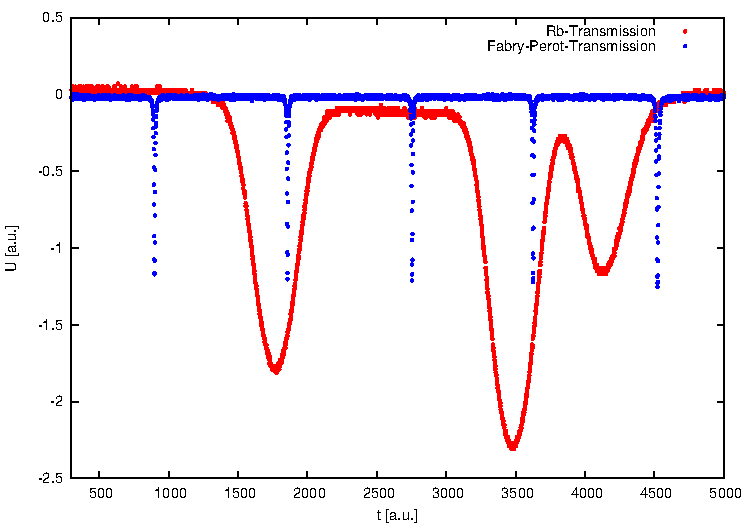
\includegraphics[width=0.9\textwidth]{./dopplerspektrum-messung.pdf}
  \caption{Die Spannung der differentiellen Photodiode (proportional zur Intensit�t
  		    des durch die Rb-Zelle transmittierten Lichts in willk�rlichen Einheiten)
			und entsprechend die Spannung hinter dem Fabry-P�rot-Resonator
		    aufgetragen gegen die Zeit $t$, w�hrend der der Frequenzbereich des Lasers 
			durchgefahren wird, ebenfalls in willk�rlichen Einheiten.}
\label{fig:dopplerroh}
\end{figure}

In Abbildung \ref{fig:dopplerroh} sind die vom Oszilloskop aufgenommenen Messdaten
dargestellt. Zu sehen sind von links nach rechts die 85F2-, 85F3- und 87F2-Resonanzen
(85F2 heisst hier z.B. die �berlagerung der drei �berg�nge vom $F=2$--Grundniveau des
$^{85}\text{Rb}$--Isotops)

Die Resonanzen des Fabry-P�rot-Signals entsprechen konstanten Frequenzabst�nden und dies
wird als Grundlage f�r einen Fit durch ein Polynom dritten Grades $f$ genutzt
(f�nf Messpunkte $(t_i,f(t_i))$ bei den Zeitpunkten $t_i$ der Resonanzen mit
gleichem $f(t)$-Abstand), siehe Abbildung \ref{fig:xumskalierung}.
\begin{figure}[!ht]
  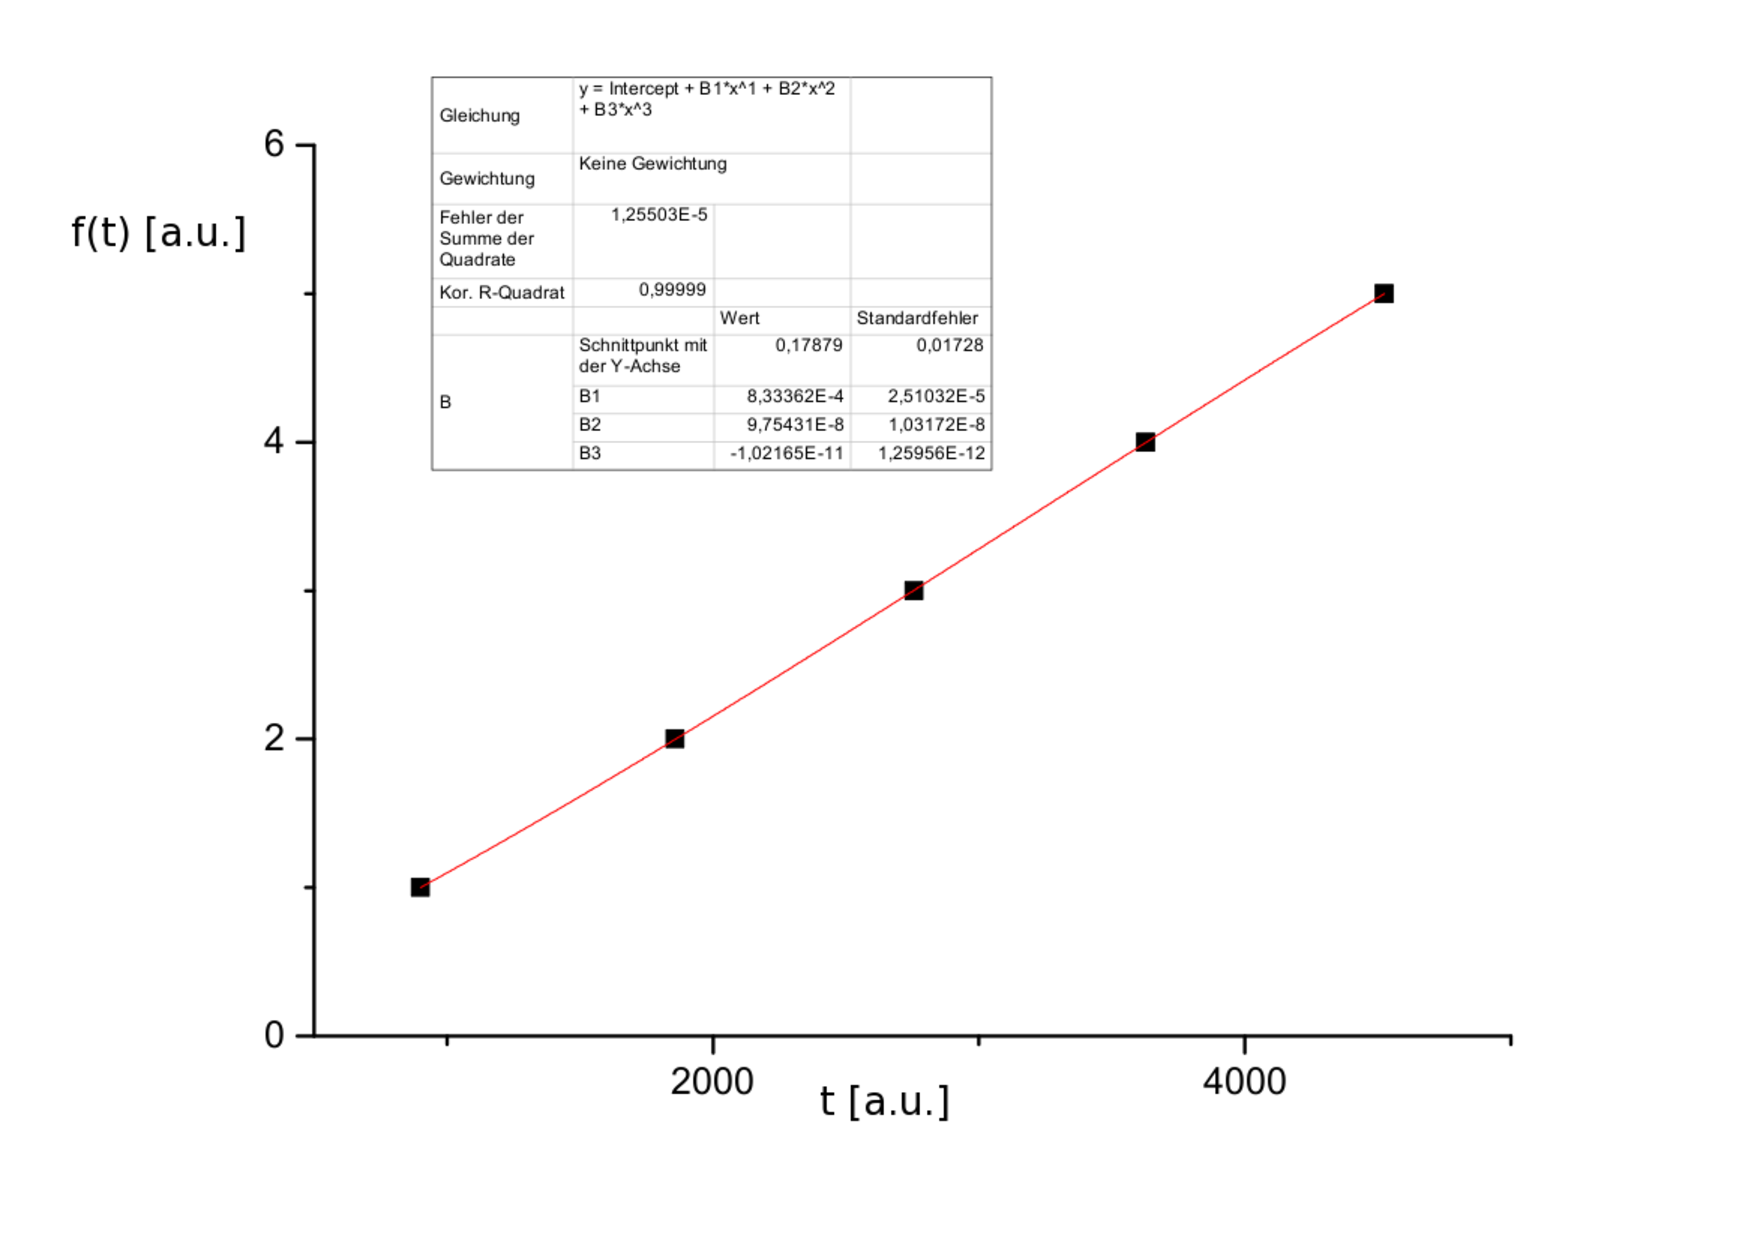
\includegraphics[width=1\textwidth]{./xumskalierung.pdf}
  \caption{Umskalierung der Messzeitachse zur Frequenzachse}
\label{fig:xumskalierung}
\end{figure}
Wenn dann das Dopplerspektrum $I$ gegen $f(t)$ aufgetragen wird, stimmt die Skalierung
bis auf eine lineare Umskalierung, die abschliessend durch Kenntnis der Position und
Abst�nde der Spektrallinien erfolgt. Vor dieser linearen Umskalierung werden die
$(I,f(t))$--Daten durch eine Summe von zwei �berlagerungen f�r die 85F2- und
85F3-Resonanzen
aus jeweils drei Gau�profilen
mit gleicher Breite (die nach \eqref{eq:gausstemp} der Temperatur des Rb-Gases entspricht)
und durch Literaturwerte [2] vorgegebene Amplitudenverh�ltnisse und einer beliebigen
Gau�funktion f�r die rechte 87F2-Resonanz gefittet.

\begin{figure}[ht]
  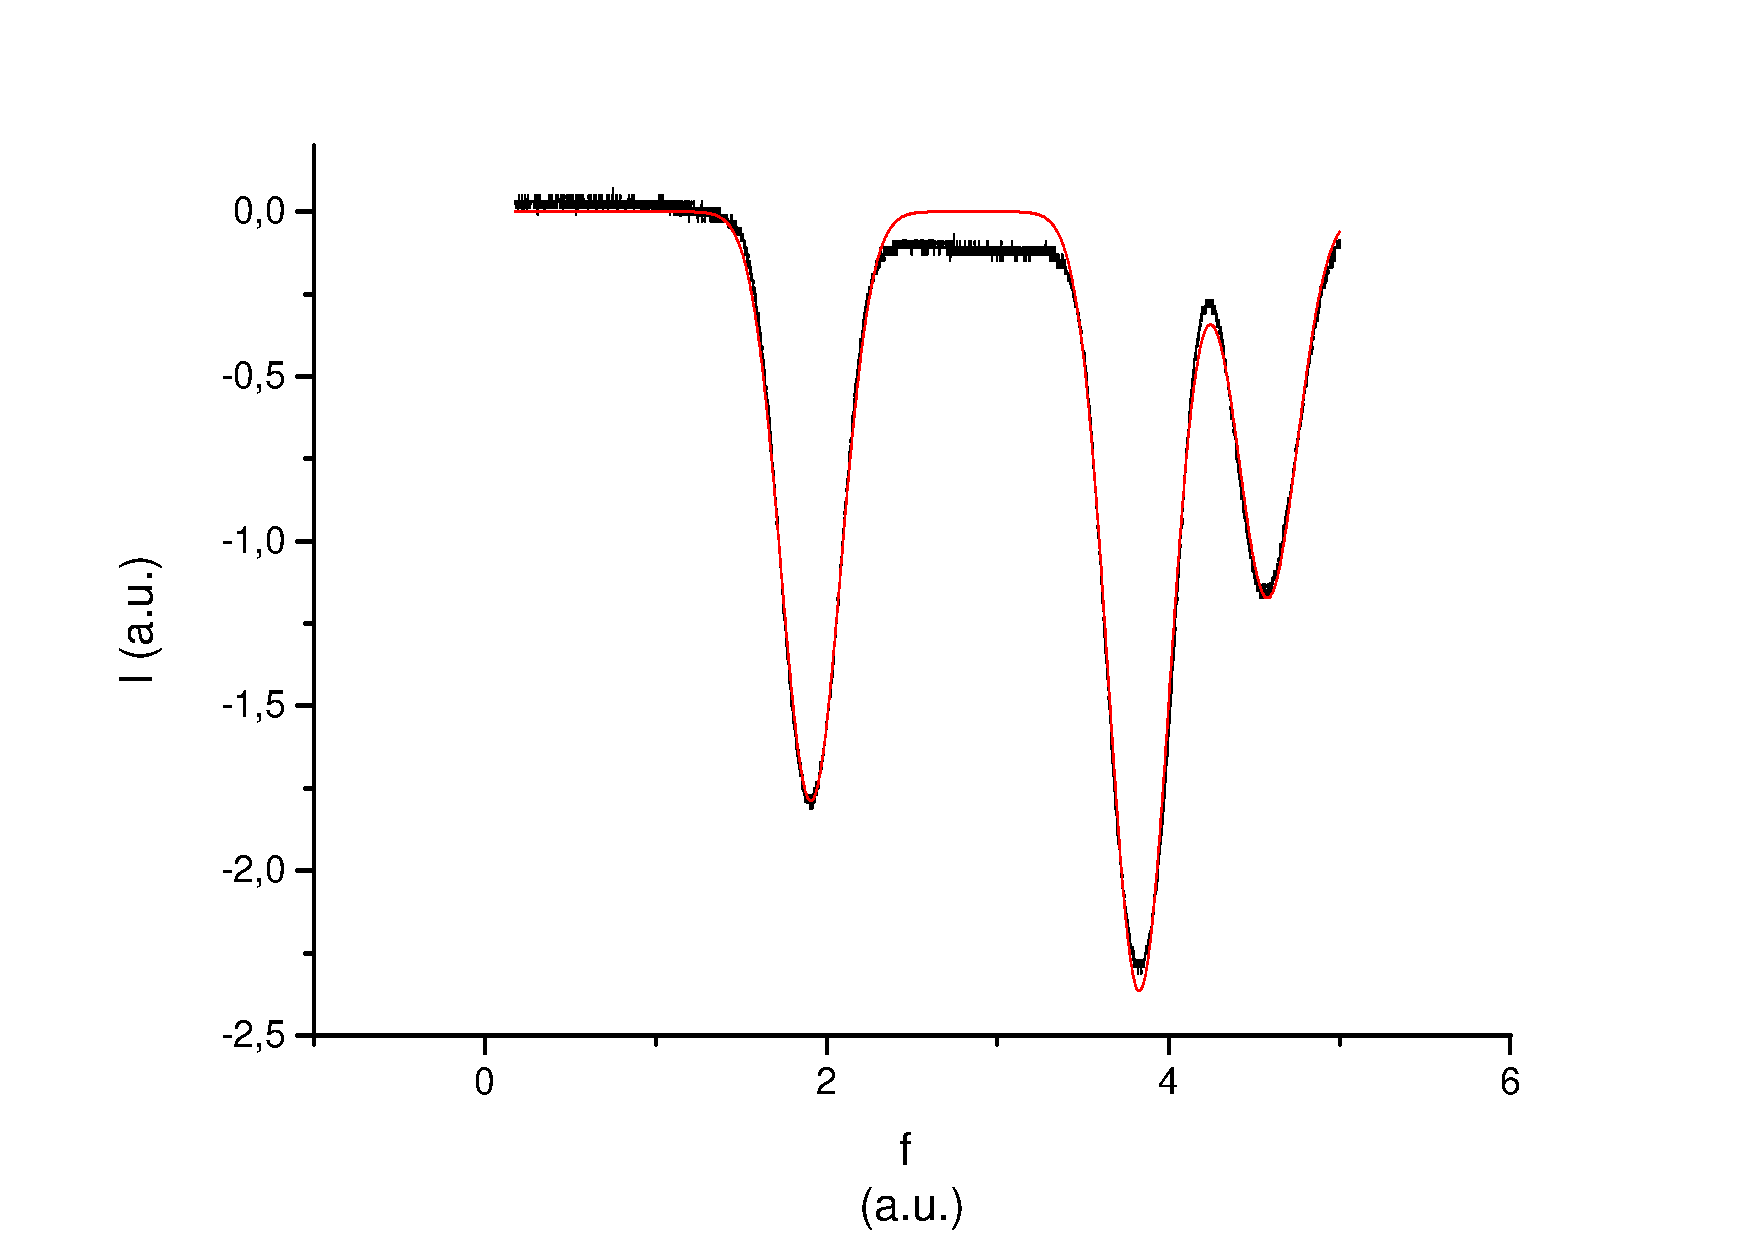
\includegraphics[width=1\textwidth]{./dopplerfit-plot.pdf}
  \caption{Gemessenes Dopplerspektrum in willk�rlichen Einheiten gegen die
  		umskalierte $f(t)$--Achse in Schwarz; Fit in Rot}
\label{fig:dopplerfit}
\end{figure}

Aus dem Fit ergibt sich eine gemeinsame halbe $\frac{1}{e}$--Breite $w$ der �berlagerten
Gau�profile f�r die 85F2- und 85F3-Resonanzen in Einheiten der $f(t)$--Achse als Parameter
des Fits, aus der
wir die volle Halbwertsbreite in MHz durch Umrechnung der Breitenarten
(halbe $\frac{1}{e}$--Breite in volle Halbwertsbreite) und
Skalierung erhalten, da die wahren relativen
Abst�nde der Resonanzen aus der Literatur [2] bekannt sind.

Wir erhalten somit:
\begin{equation}
	w = (406,5 \pm 0,8) \text{ MHz} \nonumber
\end{equation}

Mit Gleichung \eqref{eq:gausstemp} ergibt sich daraus f�r die Temperatur des Rb-Gases
\begin{equation}
	T = (434,46 \pm 1,7) \text{ K} \nonumber
\end{equation}



\section{Dopplerfreie S�ttigungsspektroskopie}

\subsection{Messung der Strahltaille}

In Abbildung \ref{fig:strahlbreite} sind die Messergebnisse der Leistungen $P_x$ und $P_y$
des durchgelassenen
Laserstrahls bei teilweiser Abdeckung durch die Rasierklinge mit Positionen $x$ aus
horizontaler Richtung bzw. $y$ aus vertikaler Richtung dargestellt. Die Nullpunkte
von $x$ und $y$ sind beliebig und irrelevant f�r die Auswertung.

Ebenfalls in Abbildung \ref{fig:strahlbreite} zu sehen sind die Fits der Messpunkte mit
Fehlerfunktionen nach \eqref{eq:yerrfct} und \eqref{eq:xerrfct}.

Aus den Fits ergeben sich die halben $\frac{1}{e^2}$--Breiten $w_x$ und $w_y$ der
als transversal gau�f�rmig verteilt angenommenen Intensit�t des Laserstrahls:

\begin{equation}
	\begin{split}
	w_x &= (1,60 \pm 0,09) \text{ mm} \\
	w_y &= (1,51 \pm 0,014) \text{ mm}
	\end{split} \nonumber
\end{equation}

\begin{figure}[!h]
  \subfigure[Strahlabdeckung aus horizontaler Richtung $x$]{
  	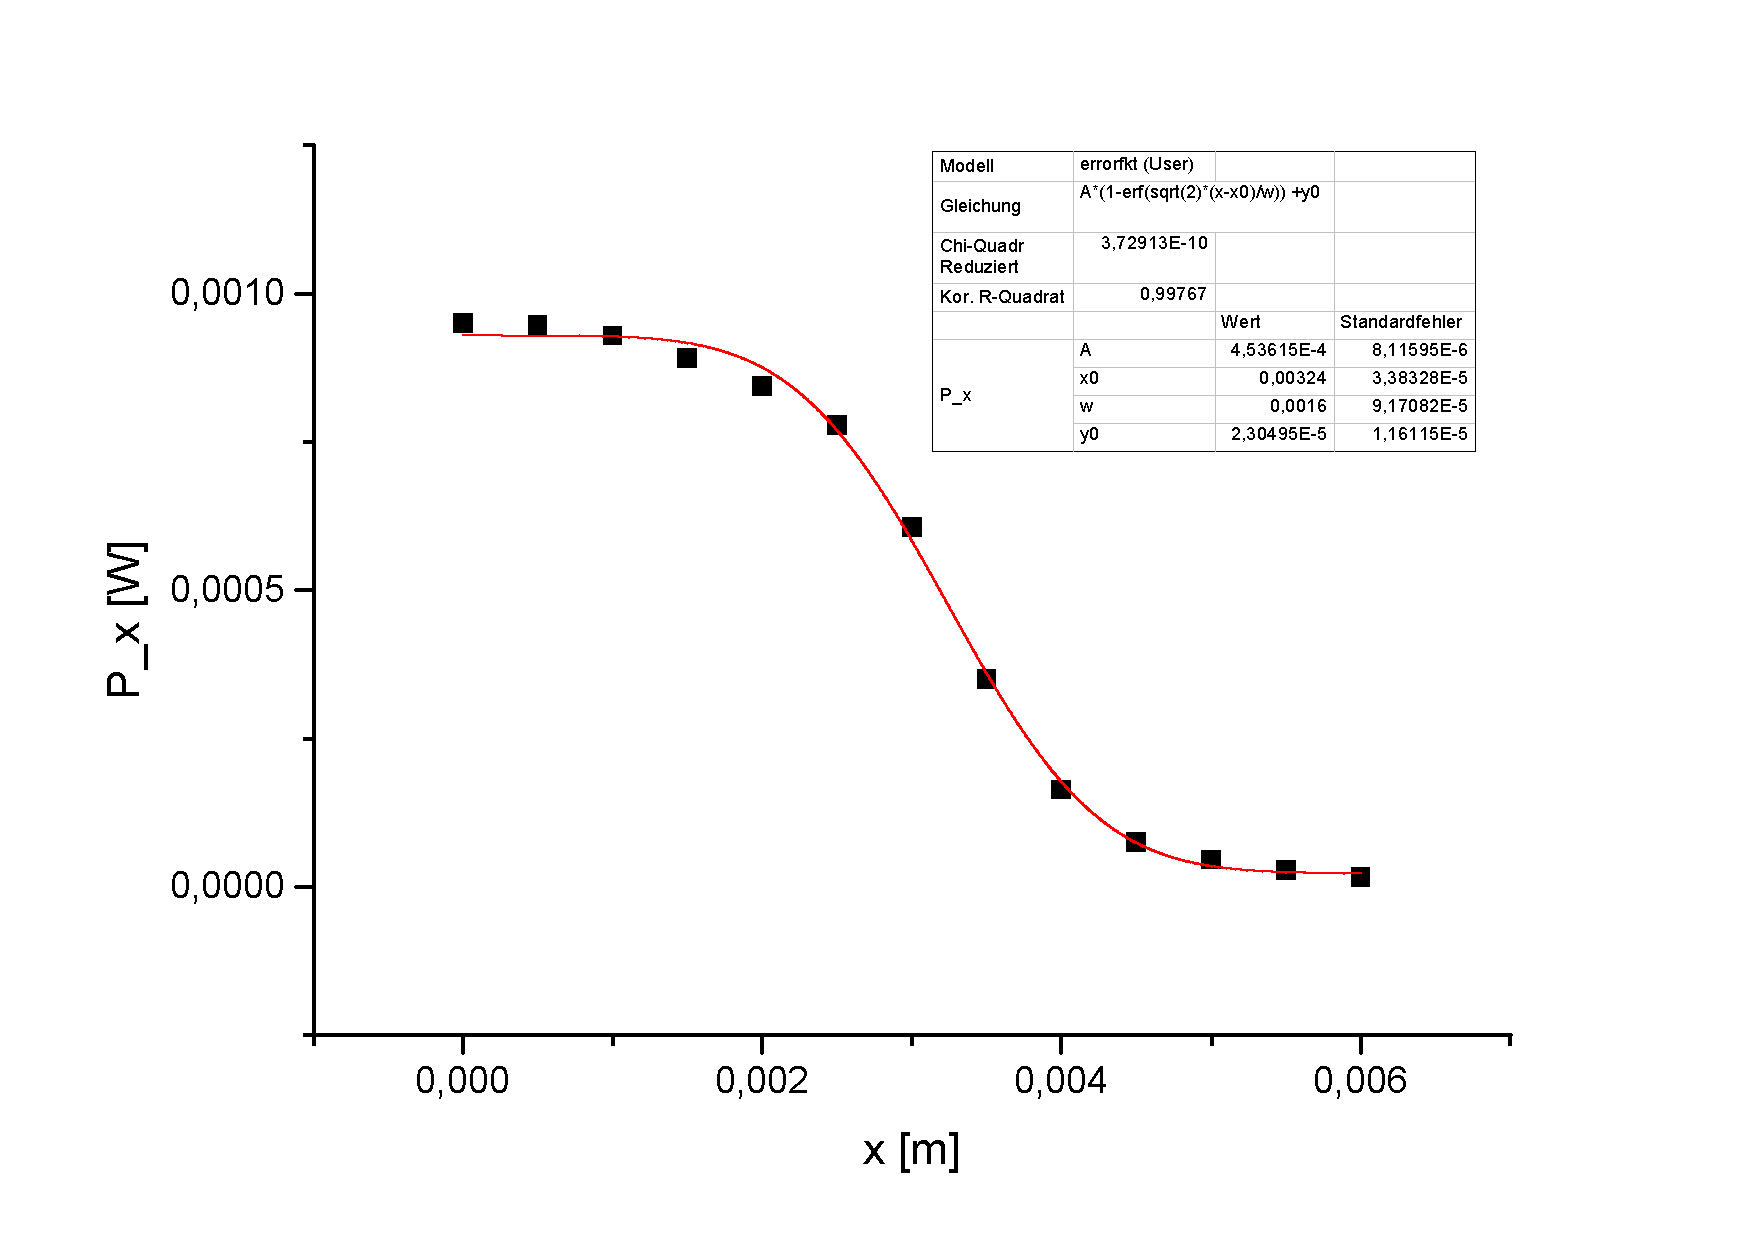
\includegraphics[width=1\textwidth]{./xstrahlbreite.pdf}
  }
  \subfigure[Strahlabdeckung aus horizontaler Richtung $y$]{
  	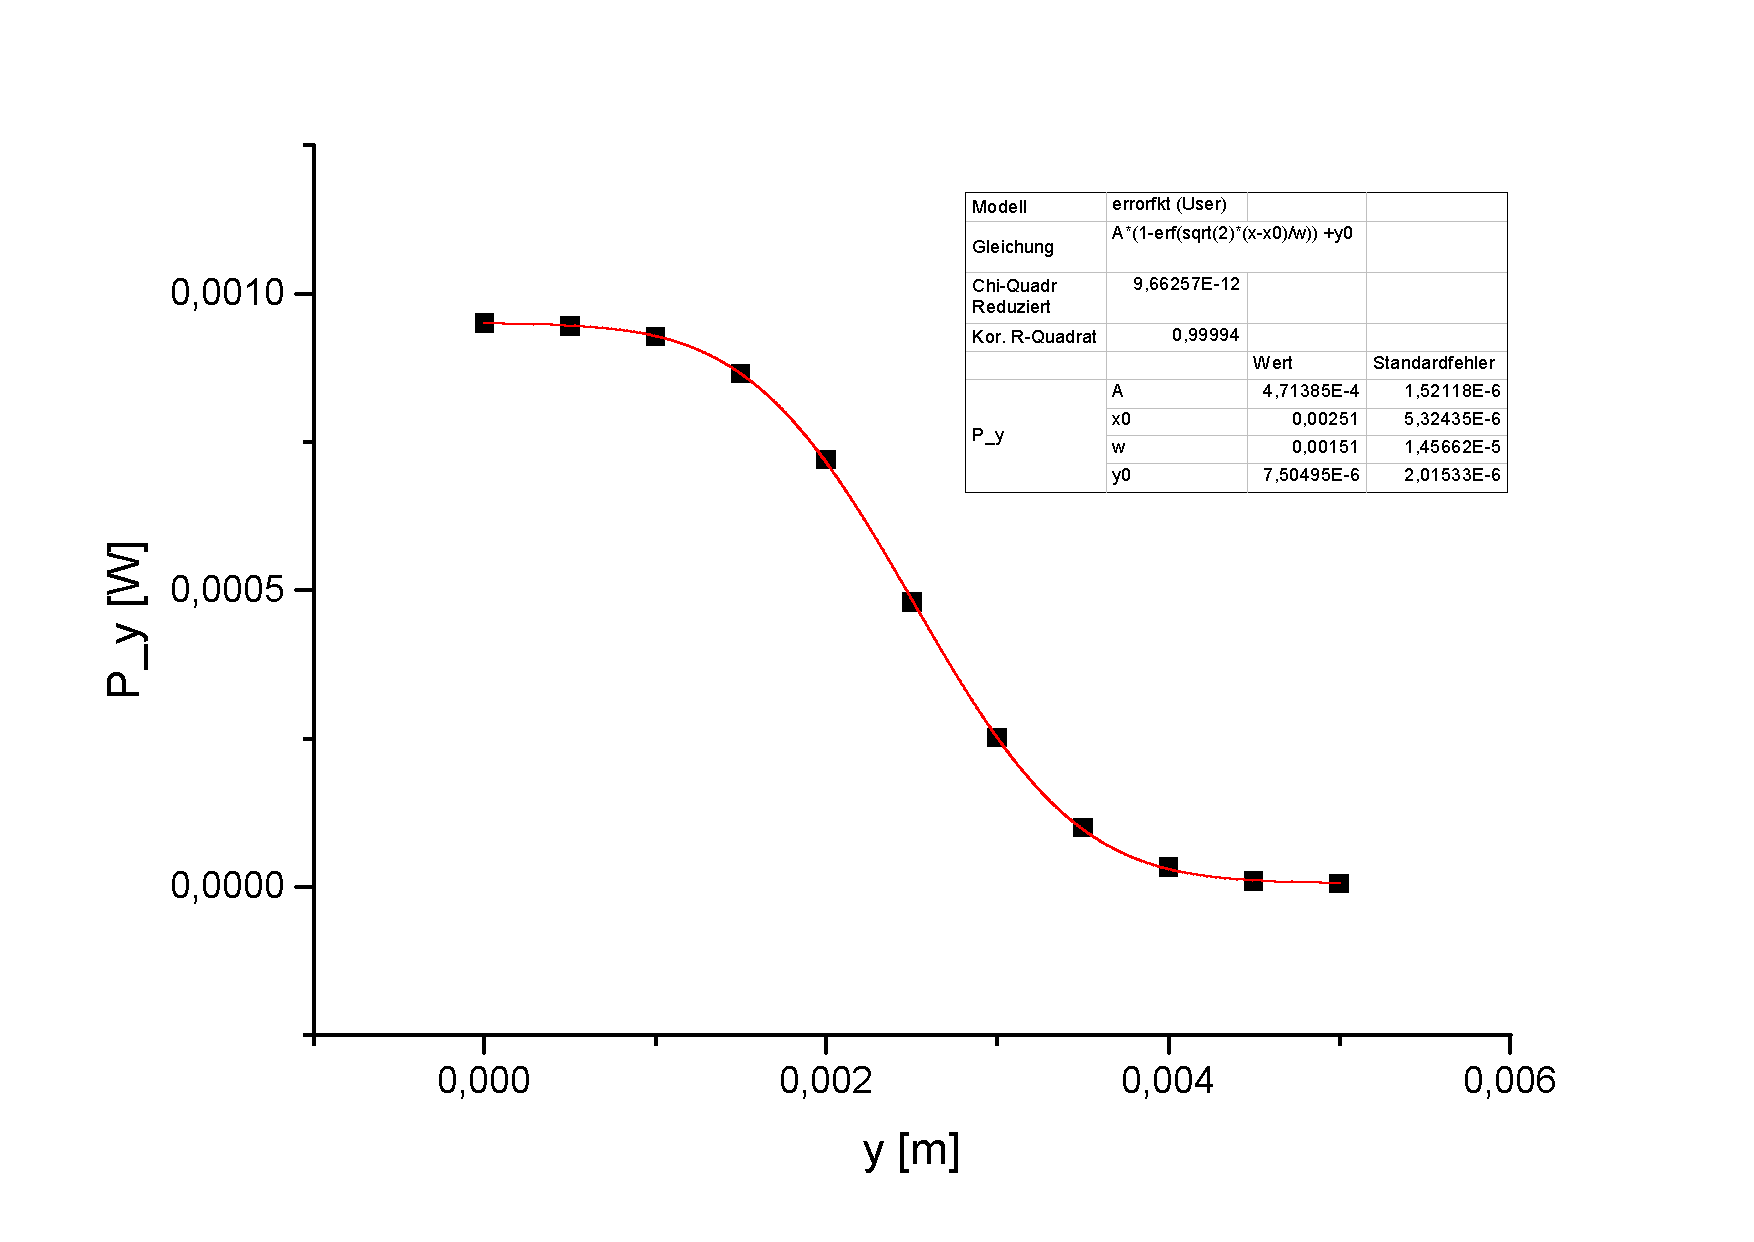
\includegraphics[width=1\textwidth]{./ystrahlbreite.pdf}
  }
  \caption{Messung der durchgelassenen Leistung bei Abdeckung durch eine Rasierklinge
  	  			in Schwarz; Fit mit Fehlerfunktion in Rot}
\label{fig:strahlbreite}
\end{figure}
\clearpage
\subsection{Bestimmung der nat�rlichen Linienbreite und S�ttigungsintensit�t}

Mithilfe der oben bestimmten Strahlbreiten $w_x$ und $w_y$ und Gleichung
\eqref{eq:intensitaet} k�nnen wir den verschiedenen Leistungen des Pumpstrahls,
zu denen wir jeweils das 87F2-Spektrum aufgenommen haben, die entsprechenden
Pumpstrahl-Intensit�ten zuordnen.
Jedes zu den verschiedenen Intensit�ten aufgenommene Spektrum wird mit
einer Summe von sechs Lorentzprofilen mit gleichen Halbwertsbreiten f�r
die drei Energie�berg�nge und die drei Crossover-Resonanzen, einer
Gau�-Funktion zur N�herung des Signaluntergrunds und einer konstanten Verschiebung gefittet.
Dabei sind die Verh�ltnisse
der Abst�nde der sechs Resonanzen aus der Literatur [2] und Theorie bekannt.
In Abbildung \ref{fig:400mukrow} ist beispielhaft die Messung bei der
Pumpstrahlleistung 400 $\mu$W zusammen mit dem Fitergebnis dargestellt.

\begin{figure}[!h]
  	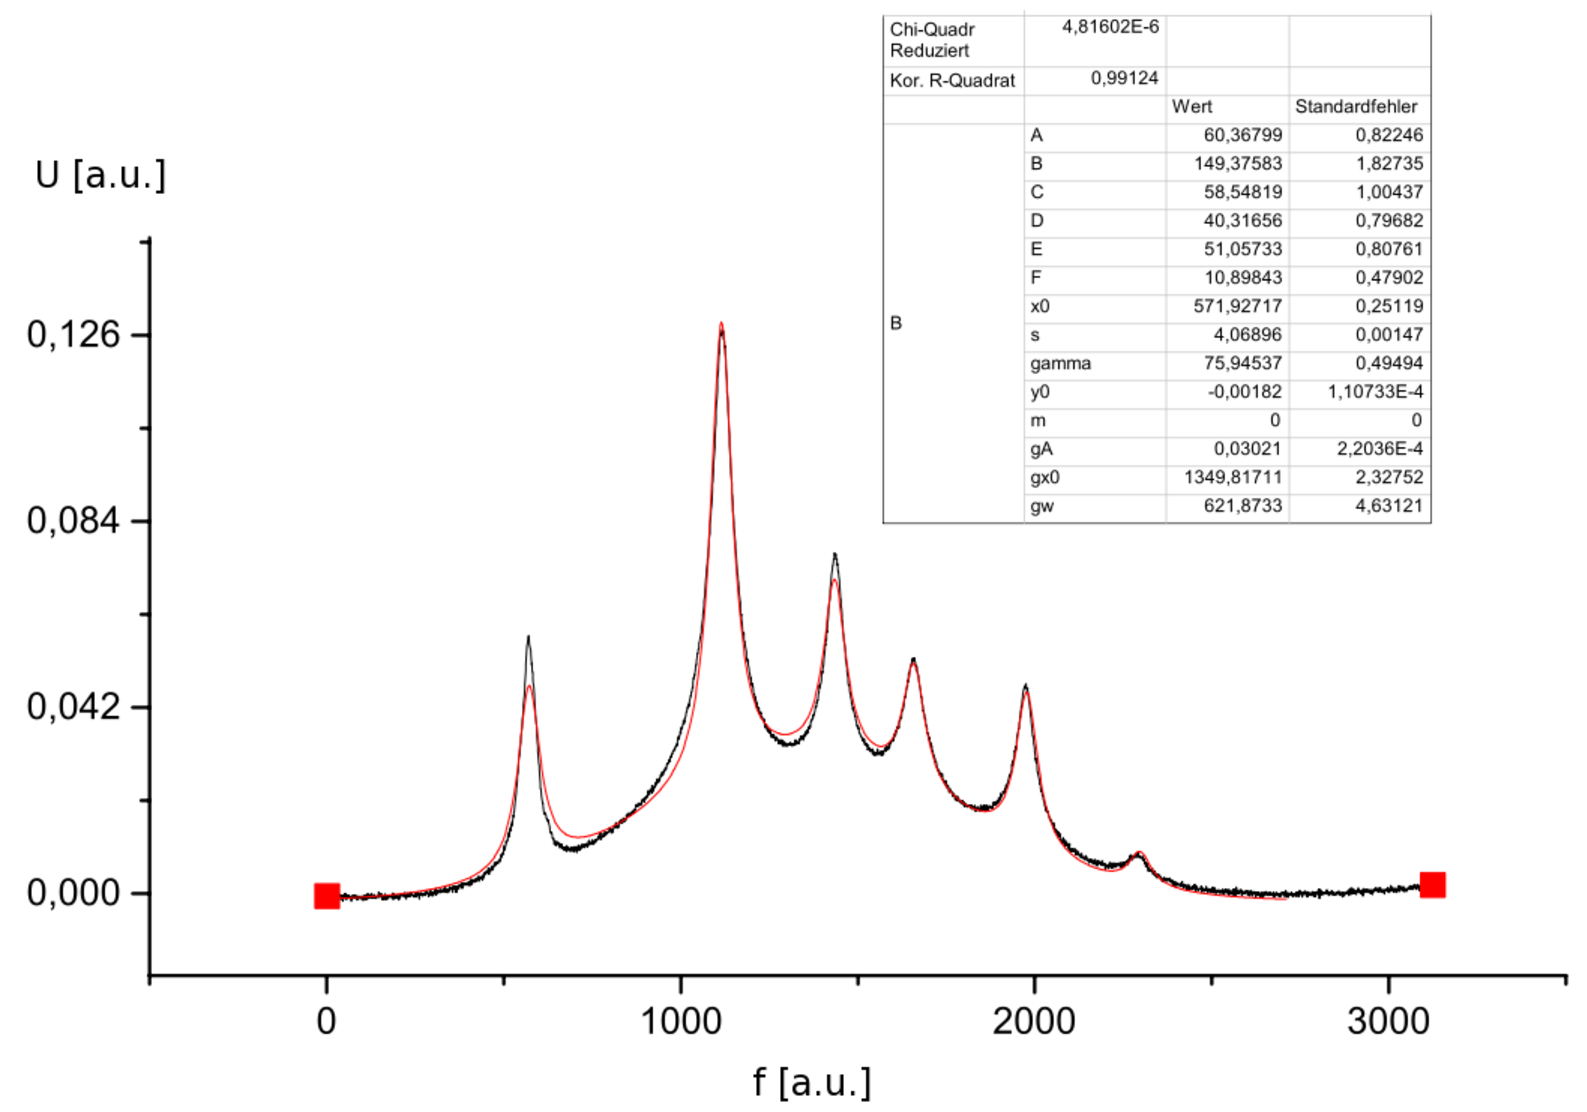
\includegraphics[width=1\textwidth]{./400uW.pdf}
  \caption{Messung der Aufspaltung der 87F2-Linie bei Pumpstrahlleistung 400 $\mu$W}
\label{fig:400mukrow}
\end{figure}

Wir erhalten also zu jeder Leistung $P$ des Pumpstrahls durch den Fit des
entsprechenden Spektrums als Parameter die volle
Halbwertsbreite $\Gamma$ der leistungsverbreiterten Resonanzen, die nach Gleichung
\eqref{eq:mitformel} von $I$ abh�ngt, welches wiederum nach \eqref{eq:intensitaet} von
$P$ abh�ngt. Durch einen Fit der Messwertepaare $(P,\Gamma)$
mit dem theoretischen Verlauf nach \eqref{eq:mitformel} und \eqref{eq:intensitaet}
werden dann die nat�rliche
Linienbreite $\gamma$ und die S�ttigungsintensit�t $I_{\text{sat}}$ von Rubidium bestimmt.
\clearpage

\begin{figure}[!h]
  	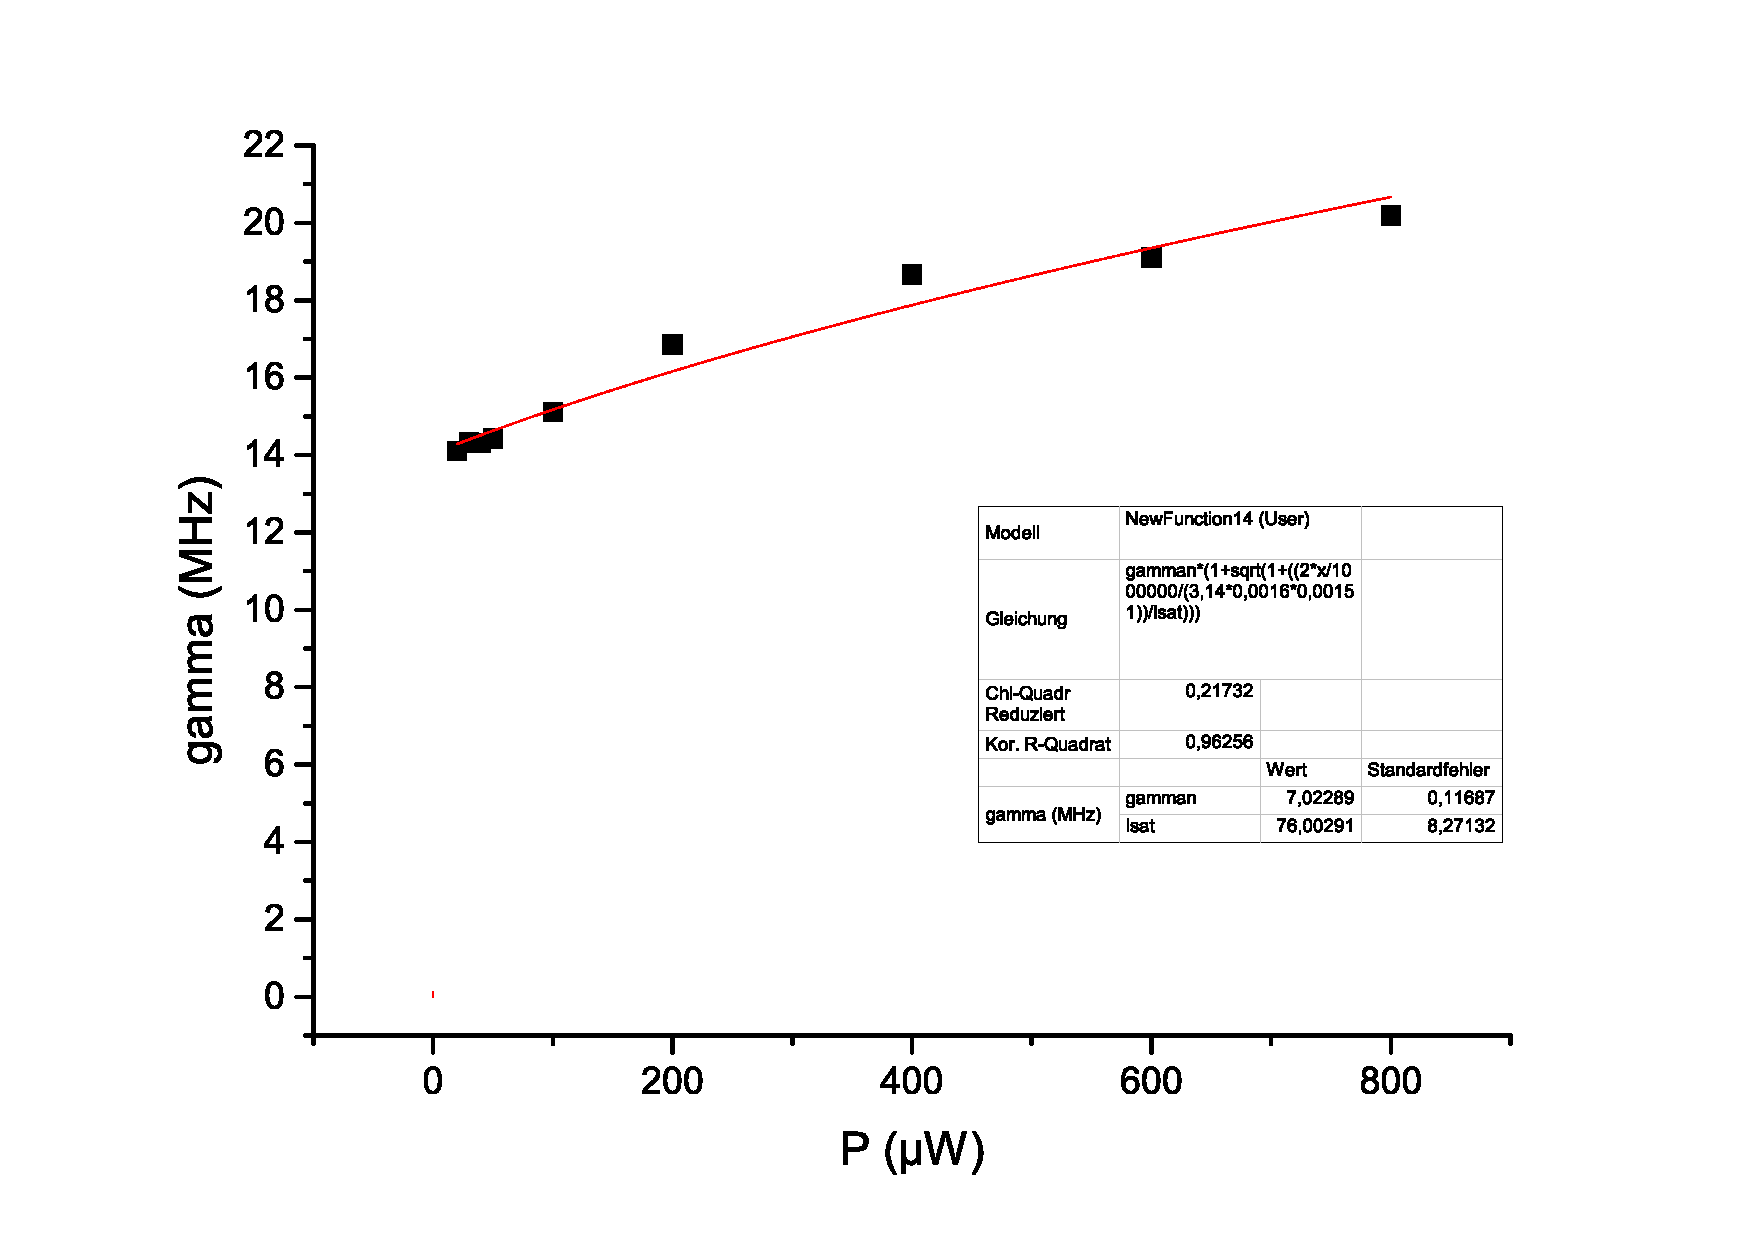
\includegraphics[width=1\textwidth]{./mitformelfit.pdf}
    \caption{Halbwertsbreiten $\Gamma$ der Lorentz-Resonanzen in Abh�ngigkeit der
			Pumpstrahlleistung $P$, Fit durch den theoretischen Verlauf
			nach \eqref{eq:mitformel}.}
\label{fig:mitformelfit}
\end{figure}
Wir erhalten:

\begin{equation}
	\begin{split}
	\gamma &= (7,02 \pm 0,12) \text{ MHz} \\
	I_{\text{sat}} &= (7,6 \pm 0,8) \frac{\text{mW}}{\text{cm}^2}
	\end{split} \nonumber
\end{equation}

\begin{figure}[!h]
  \subfigure[alle]{
  	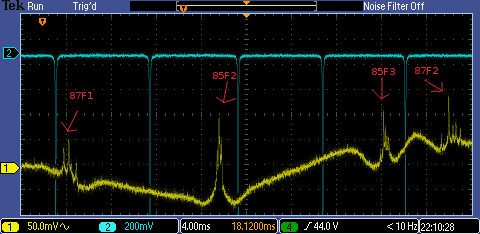
\includegraphics[width=1\textwidth]{./alle.png}
  } \\
  \subfigure[87F1]{
  	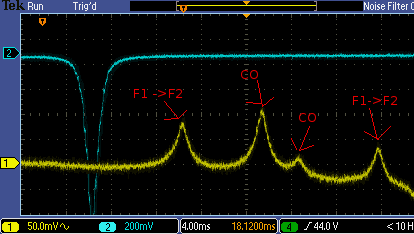
\includegraphics[width=0.5\textwidth]{./87F1.png}
  }
  \subfigure[85F2]{
  	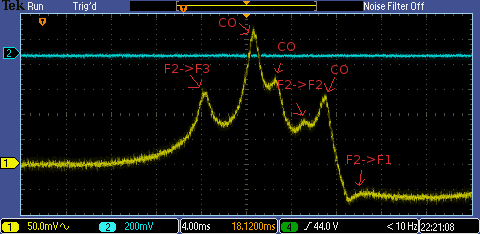
\includegraphics[width=0.5\textwidth]{./85F2.png}
  } \\
  \subfigure[85F3]{
  	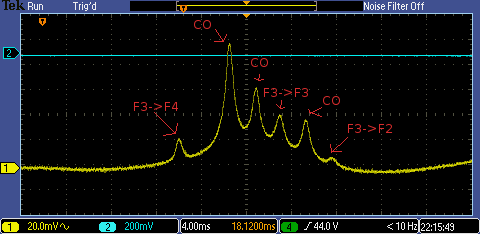
\includegraphics[width=0.5\textwidth]{./85F3.png}
  }
  \subfigure[87F2]{
  	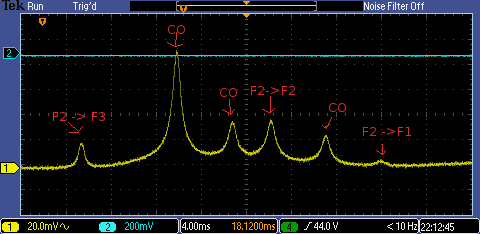
\includegraphics[width=0.5\textwidth]{./87F2.png}
  } \\
  \caption{Identifizierung der Hyperfeinstrukturlinien und der Crossover-Resonanzen}
\label{fig:identifi}
\end{figure}
\chapter{Fehlerdiskussion}
\section{Dopplerverbreitertes Spektrum}
Wir hatten gehofft �ber die $\frac{1}{e}$--Breite $w$ der Gau�fits im dopplerverbreitertem Spektrum auf die Temperatur des Rb-Gases zu schlie�en.
Erwartet h�tten wir, dass das Gas ungef�hr die Raumtemperatur von ca. 300 K bwz. 20-30�C angenommen hat, stattdessen haben wir einen errechneten Wert von
\begin{equation}T = (434,46 \pm 1,7) \text{ K} \nonumber
 \end{equation}
 
Dieser Wert liegt nat�rlich jenseits jeder Vernunft. W�re die Rb-Zelle wirklich so hei� gewesen, h�tten wir sie gar nicht ohne Verbrennungen mit blo�er Hand 
anfassen k�nnen. 

Wir k�nnen uns leider nicht erkl�ren wieso wir eine derart gro�e Abweichung vom erwarteten Wert erzielt haben, vorallem wenn wir mit 6 Gau�profile gefittet 
haben und trotzdem nur einen kleinen Fehler rausbekommen haben. Dies deutet auf einen gro�es systematischen Fehler hin vielleicht in der theoretischer Vorhersage.
�ber den Zusammenhang der Breite und Temperatur.

--------

Der von uns experimentell ermittelte Wert f�r die Temperatur der Rubidiumzelle betr�gt
\begin{equation}
	T = (434,46 \pm 1,7) \text{ K} \nonumber
\end{equation} 
Dieser Wert weicht nat�rlich stark von der erwarteten Raumtemperatur ab.
Dass wir sechs verschiedene dopplerverbreiterte Resonanzen f�r den Fit verwendet haben
und f�r die Halbwertsbreite trotzdem nur einen kleinen Fehler rausbekommen haben, k�nnte
auf einen systematischen Fehler hindeuten, der vielleicht aus der theoretischen Vorhersage
�ber den Zusammenhang der Linienbreite und der Temperatur herr�hrt.

\section{Dopplerfreie S�ttigungsspektroskopie}

Um die Leistung des Pumpstrahls �ber seine \(\frac{1}{e^2}\)-Breite in Intensit�t umzurechnen,
haben wir die Formel 
in \eqref{eq:intensitaetleistung} verwendet. Wie schon im dem theoretischen Teil beschrieben ist diese Formel jedoch eine grobe N�herung, da man zuerst von einer gau�verteilten Intensit�t
ausgeht, aber dann annimmt die Intensit�t w�re konstant gleich der Amplitude \(I_0 \) der Gau�funktion.
Das f�hrt zu einer �bersch�tzung der S�ttigungsintensit�t und kann teilweise erkl�ren,
wieso der gemessene Wert gr��er als der Literaturwert [2] ist.

\begin{equation}
	\begin{split}
	 I_{\text{sat},exp} &= (7,6 \pm 0,8) \frac{\text{mW}}{\text{cm}^2} \\
	  I_{\text{sat},theo} &= 1,6\frac{\text{mW}}{\text{cm}^2}                                    
	\end{split} \nonumber
\end{equation}

Um sich dem theoretischen Model besser anzun�hern, k�nnte man mit Blenden arbeiten,
mit denen man die R�nder der Gau�funktion abschneidet, um somit
den Unterschied zwischen gau�verteilter und konstanter Funktion zu senken.

Wir mussten bei der Aufnahme der 87F2-Linien mehrere Male die Messung wiederholen, da wir mit einem sehr starken gau�verteilten Untergrund zu k�mpfen hatten, 
den wir uns zun�chst nicht erkl�ren konnten. Er kam dem Effekt nahe, den wir im ersten Versuchsteil gemessen haben
und den wir mit dem Referenzstrahl eigentlich kompensieren wollten. Mysteri�ser wurde es, als sich der Effekt verst�rkte, je h�her die Leistung
am Pumpstrahl eingestellt wurde. 


Es stellte sich heraus, dass Reflexionen des Pumpstrahls an den R�ndern der Rubidiumzelle daf�r verantwortlich waren. 

Wir haben das Ger�st in einem gr��eren Winkel schr�g zum Pumpstrahl, wie in \ref{fig:dopplerfrei} illustriert, gestellt
 damit die Reflexionen nicht mehr in die Photodiode trafen.

Dies hat die Messung erheblich vereinfacht und verbessert. Nat�rlich k�nnen wir empfehlen ein weniger spiegelndes Material zu verwenden,
nur ist das in der Arbeit mit optischen Gegenst�nden selbstverst�ndlich. Alternativ k�nnte man einen dritten Referenzstrahl bzw. 
die Reflexionen des Pumpstrahles in Abh�ngigkeit von dessen Leistung separat aufnehmen und das als Hintergrundrauschen mitbeachten.
% Literaturverzeichnis mit File literatur.tex
\chapter{Literaturverzeichnis}

\begin{flushleft}
[1] \textit{Unbekannter Autor}. F-Praktikum: Modern Methods in Laser
	Spectroscopy, Institut f�r Laserphysik der Universit�t Hamburg.

[2] \textit{Jula Draeger, Martin Beye}. Laserspektroskopie in Rubidium
-- Dopplerprofile, Subdopplerspektren durch S�ttigungsspektroskopie und
Dunkelresonanzen, Studienarbeit am Institut f�r Laserphysik der Universit�t Hamburg.
\end{flushleft}

\end{document}

